%==============================================================================
%  Final Project Paper -- IEEE Conference format (padp-final-templates)
%  Project Category B: AI-agent code optimization.
%==============================================================================
\documentclass[conference]{IEEEtran}
\IEEEoverridecommandlockouts

\usepackage[utf8]{inputenc}
\usepackage{cite}
\usepackage{amsmath,amssymb,amsfonts}
\usepackage{graphicx}
\usepackage{booktabs}
\usepackage{multirow}
\usepackage{textcomp}
\usepackage{xcolor}
\usepackage{listings}
\usepackage{tikz}
\usetikzlibrary{arrows.meta, positioning, calc}
\usepackage{url}
\usepackage[hidelinks]{hyperref}

% --- page-budget check (per template): records where body+refs end.
\newcommand{\mainbodyendpage}{?}
\AtEndDocument{%
  \typeout{====================================================}%
  \typeout{[PAGE BUDGET] Main body + references end on page \mainbodyendpage\space (limit: 6, Appendix excluded).}%
  \typeout{====================================================}%
}

\lstset{
  basicstyle=\ttfamily\footnotesize,
  breaklines=true, frame=single, columns=fullflexible,
  showstringspaces=false, keepspaces=true, xleftmargin=0.5em,
  extendedchars=true, inputencoding=utf8,
  literate={—}{{---}}1 {–}{{--}}1 {→}{{$\rightarrow$}}1
           {≈}{{$\approx$}}1 {×}{{$\times$}}1 {≥}{{$\geq$}}1
}

\begin{document}

\title{An LLM Tree-Search Harness for Triton GPU Kernel Optimization:\\
Two Generation Engines on a 17-Operator Suite\\
{\footnotesize Final Project --- Parallel Programming, Spring 2026}}

\author{%
\hfil
\parbox[t]{0.31\textwidth}{\centering Wei-Ke Chu\\ \footnotesize R13922198\\
  Computer Science and Information Engineering\\ National Taiwan University\\
  abat52875@gmail.com}%
\hfil
\parbox[t]{0.31\textwidth}{\centering Ju-Hsuan Wang\\ \footnotesize R13945026\\
  Biomedical Electronics and Bioinformatics\\ National Taiwan University}%
\hfil
\parbox[t]{0.31\textwidth}{\centering Wen-An Wen\\ \footnotesize R13944053\\
  Computer Science and Information Engineering\\ National Taiwan University}%
\hfil
}

\maketitle

\begin{abstract}
We study whether large language models (LLMs) can optimize parallel GPU kernels,
and which \emph{kind} of LLM driver suits which kind of problem. We build a
closed-loop harness in which an LLM proposes Triton kernels, a fixed evaluator
compiles, checks, and times each candidate in an isolated subprocess, and a beam
search expands the best correct candidates. Two generation engines share the one
evaluator: an automated API loop driven by \textsc{DeepSeek-v4-flash}, and an
agentic loop in which \textsc{Claude Code} writes and repairs kernels over several
reasoning steps. We deliberately include hard kernels the cheap loop cannot solve
and design a handoff contract (\texttt{HARNESS.md}) that routes them to the agent,
specifying what it reads, writes, and its iteration budget. On a 17-operator suite benchmarked against PyTorch eager on an
NVIDIA RTX~5090, the API loop reaches $4.6\times$ on KL-divergence and
$2.2$--$4.3\times$ on RoPE, Welford, RMSNorm, and cross-entropy, while honestly
reporting $\approx 1.0\times$ on five operators already at the memory roofline.
The same engine fails completely on the hardest compute-bound problem, 4-bit
weight GEMM: 0 of 12 candidates compiled to a correct kernel, and scaling the
generator to the larger \textsc{DeepSeek-v4-pro} does not fix it (still 0/12). The
agentic engine solved it to $1.09\times$ over a cuBLAS-plus-dequantize baseline,
and reached about $5\times$ on fused-linear cross-entropy, another compute-bound
problem the API loop could not crack. The engines are complementary. Every number is derived mechanically from per-candidate run logs
at a total LLM cost of \$0.22. Code, run logs, and the scripts that regenerate
every figure and table are available at
\textcolor{blue}{\url{https://github.com/abattada/Tree-Harness-Kernel-Optimization}}.
\end{abstract}

\begin{IEEEkeywords}
GPU kernels, Triton, LLM code generation, AI agents, performance optimization,
roofline
\end{IEEEkeywords}

\vspace{0.3em}
\noindent\textbf{Project category.} This is a \textbf{Category~B} project
(AI-agent code optimization): we optimize parallel GPU kernels with two
LLM-driven engines and analyze, in particular, the cases where the agents fail.

%------------------------------------------------------------------------------
\section{Introduction}
Writing fast GPU kernels is expensive expert labor. A kernel's performance hinges
on tiling, vectorization, memory-access patterns, and launch parameters
(block sizes, warps, pipeline stages), and the interaction of these choices is
hard to predict. We ask whether large language models can do this optimization,
and---the sharper question---\emph{which style of LLM driver fits which kind of
kernel}. We compare a cheap, high-throughput API loop against an agentic loop
that can reason across steps and repair its own errors.

We built a closed-loop harness that treats kernel optimization as an
LLM-in-the-loop tree search over Triton~\cite{tillet2019triton} implementations.
Candidate code never touches the clock: all timing and correctness checking live
in a fixed evaluator, so reported speedups are defensible. Two generation engines
plug into that one evaluator. A central design choice is that the suite
\emph{deliberately} includes hard, compute-bound kernels that the cheap one-shot
loop cannot solve, together with a contract (\texttt{HARNESS.md}) that hands those
operators to an agent able to iterate. Our contributions are (i) a reproducible
harness with a strict provenance discipline; (ii) \emph{a designed agent-handoff
contract} (Fig.~\ref{fig:harness}) that routes the operators the API loop fails on
to an agentic LLM, specifying exactly what the agent reads, what it writes, and
its iteration budget, so both engines feed one comparison pipeline; and (iii) an
honest result---the API loop, even scaled to a larger model, cannot solve the hard
compute-bound kernels (\texttt{int4\_gemm}, \texttt{flce}) that the agent solves,
to near hardware peak and $\sim$5$\times$ respectively.

%------------------------------------------------------------------------------
\section{Background and Related Work}
\textbf{Benchmark and baseline.} Our suite has 17 operators across elementwise,
reduction, normalization, loss, matmul, and positional categories, chosen to
mirror the Liger operator family~\cite{hsu2024liger} used in LLM training. The
baseline for every operator is PyTorch \emph{eager} execution of a reference
implementation; the kernel's job is to match the reference within tolerance and
run faster. Twelve operators have optimization headroom; five
(\texttt{vector\_add}, \texttt{vector\_exp}, \texttt{sum}, \texttt{softmax},
\texttt{layer\_norm}) already saturate memory bandwidth and serve as a control
group. We use the full suite, not a subset.

\textbf{LLMs for kernels.} KernelBench~\cite{ouyang2025kernelbench} asks whether
LLMs can write efficient GPU kernels and reports that correctness, not just
speed, is the binding constraint. Production libraries such as
Liger~\cite{hsu2024liger} show that a small set of fused Triton kernels removes
most intermediate-tensor traffic in training; the largest wins come from the same
idea we exploit---fusing multi-pass references into a single pass.

\textbf{Agent setup.} Engine~A calls \textsc{DeepSeek-v4-flash} (thinking
enabled) through an OpenAI-compatible API. Engine~B is \textsc{Claude Code}
(model \textsc{Claude Opus}, reasoning effort ``extra high'') operating under a
written contract (\texttt{HARNESS.md}) that lets it write a kernel, invoke the
evaluator, read the traceback or measurement, and iterate. The verbatim prompts
and configuration are in the Appendix.

%------------------------------------------------------------------------------
\section{Methodology}
\subsection{Closed loop and the two engines}
Fig.~\ref{fig:pipeline} shows the harness. It seeds an initial population from
design hints, asks the LLM to emit a Triton module exposing
\texttt{triton\_run(*inputs)}, evaluates each candidate, scores the correct ones
against a roofline anchor, and expands a top-$k$ beam into the next round. A
knowledge base (KB) of previously winning kernels is retrieved as few-shot
exemplars and rebuilt from the logs between batches.

\begin{figure*}[t]
  \centering
  \resizebox{0.95\textwidth}{!}{% TikZ architecture figure for the closed-loop harness and the two engines.
% % TikZ architecture figure for the closed-loop harness and the two engines.
% % TikZ architecture figure for the closed-loop harness and the two engines.
% \input{make_pipeline_fig.tex} inside a figure environment in REPORT.tex.
% Layout uses explicit coordinates and routes every feedback line through an
% empty band so no arrow ever crosses a box.
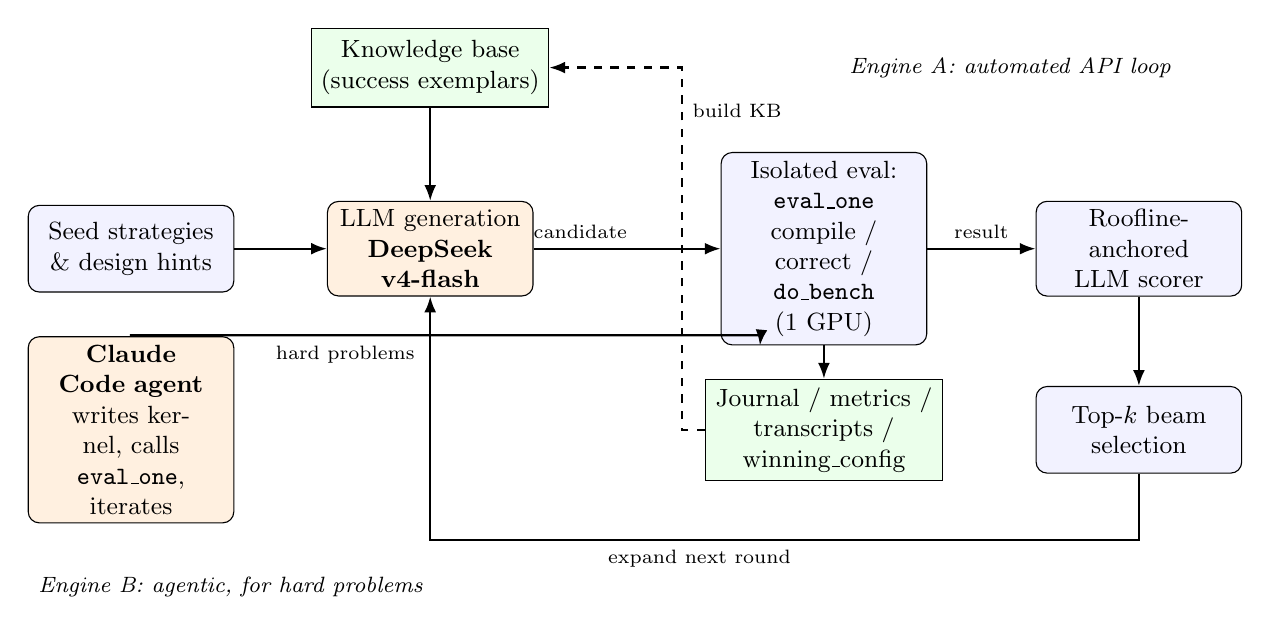
\begin{tikzpicture}[
    font=\small,
    box/.style={draw, rounded corners, align=center, text width=24mm,
                minimum height=11mm, inner sep=3pt, fill=blue!5},
    eng/.style={draw, rounded corners, align=center, text width=24mm,
                minimum height=11mm, inner sep=3pt, fill=orange!12},
    store/.style={draw, align=center, text width=28mm, minimum height=10mm,
                  inner sep=3pt, fill=green!8},
    arr/.style={-{Latex[length=2mm]}, thick},
  ]

  % main row (y=0); eval/score pushed right to lengthen the gen->eval arrow
  \node[box] (seed)  at (0,0)     {Seed strategies \\ \& design hints};
  \node[eng] (gen)   at (3.8,0)   {LLM generation \\ \textbf{DeepSeek v4-flash}};
  \node[box] (eval)  at (8.8,0)   {Isolated eval: \texttt{eval\_one} \\ compile / correct / \\ \texttt{do\_bench} (1 GPU)};
  \node[box] (score) at (12.8,0)  {Roofline-anchored \\ LLM scorer};

  % satellites
  \node[store] (kb)   at (3.8,2.3)  {Knowledge base \\ (success exemplars)};
  \node[store] (jrn)  at (8.8,-2.3) {Journal / metrics / \\ transcripts / winning\_config};
  \node[box]   (beam) at (12.8,-2.3){Top-$k$ beam \\ selection};
  \node[eng]   (agent) at (0,-2.3)  {\textbf{Claude Code agent} \\ writes kernel, calls \\ \texttt{eval\_one}, iterates};

  % straight links; "candidate" sits on the LEFT of the (now longer) arrow
  \draw[arr] (seed) -- (gen);
  \draw[arr] (gen)  -- node[above,font=\scriptsize,pos=0.25]{candidate} (eval);
  \draw[arr] (eval) -- node[above,font=\scriptsize]{result} (score);
  \draw[arr] (kb)   -- (gen);
  % eval -> journal leaves from the CENTER-bottom of eval
  \draw[arr] (eval.south) -- (jrn.north);
  \draw[arr] (score) -- (beam);

  % beam -> gen feedback ("expand"): down, left along the lowest band, up into gen
  \draw[arr] (beam.south) -- (12.8,-3.7) -- node[below,font=\scriptsize,pos=0.62]{expand next round}
        (3.8,-3.7) -- (gen.south);

  % journal -> KB feedback (dashed): up the RIGHT part of the gen--eval gap (x=7.0)
  \draw[arr,dashed] (jrn.west) -- (7.0,-2.3) -- node[right,font=\scriptsize,pos=0.88]{build KB}
        (7.0,2.3) -- (kb.east);

  % Claude agent -> eval ("hard problems"): across an empty band (y=-1.1) into the
  % SOUTH-WEST corner of eval, so it does not share the eval->journal start point.
  \draw[arr] (agent.north) -- (0,-1.1) -- node[below,font=\scriptsize,pos=0.34]{hard problems}
        (8.0,-1.1) -- ([xshift=5mm]eval.south west);

  % engine labels, clear of every box and routed line
  \node[font=\footnotesize\itshape, anchor=west] at (9.0,2.3)  {Engine A: automated API loop};
  \node[font=\footnotesize\itshape, anchor=west] at (-1.3,-4.3) {Engine B: agentic, for hard problems};

\end{tikzpicture}
 inside a figure environment in REPORT.tex.
% Layout uses explicit coordinates and routes every feedback line through an
% empty band so no arrow ever crosses a box.
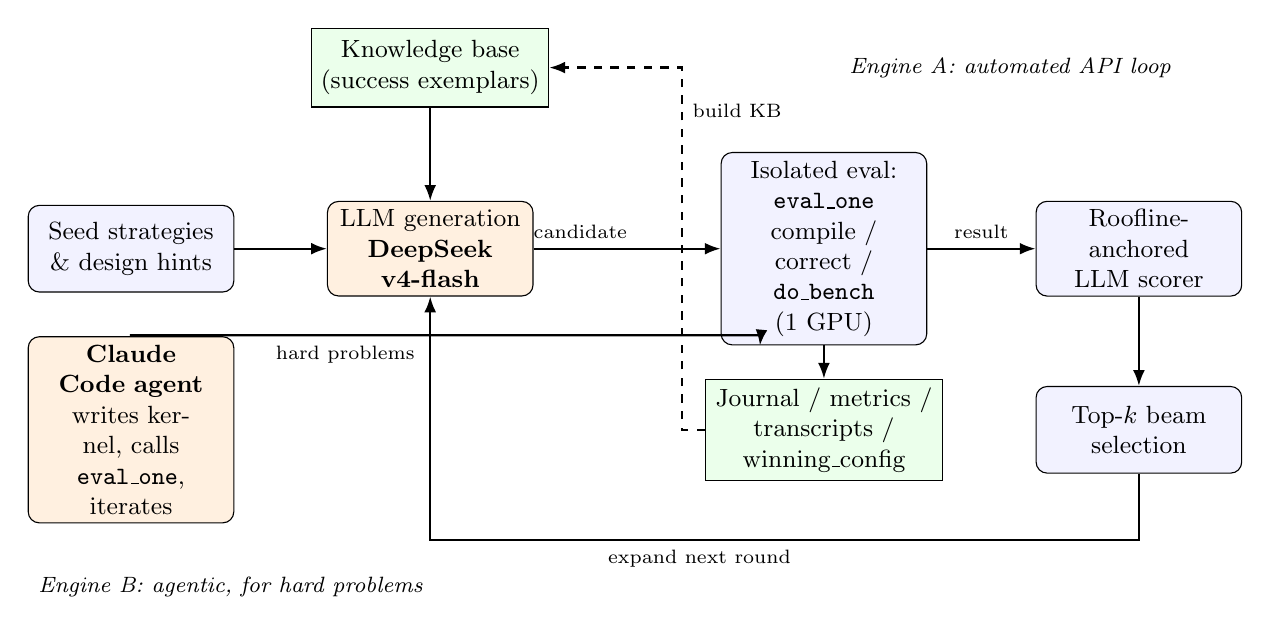
\begin{tikzpicture}[
    font=\small,
    box/.style={draw, rounded corners, align=center, text width=24mm,
                minimum height=11mm, inner sep=3pt, fill=blue!5},
    eng/.style={draw, rounded corners, align=center, text width=24mm,
                minimum height=11mm, inner sep=3pt, fill=orange!12},
    store/.style={draw, align=center, text width=28mm, minimum height=10mm,
                  inner sep=3pt, fill=green!8},
    arr/.style={-{Latex[length=2mm]}, thick},
  ]

  % main row (y=0); eval/score pushed right to lengthen the gen->eval arrow
  \node[box] (seed)  at (0,0)     {Seed strategies \\ \& design hints};
  \node[eng] (gen)   at (3.8,0)   {LLM generation \\ \textbf{DeepSeek v4-flash}};
  \node[box] (eval)  at (8.8,0)   {Isolated eval: \texttt{eval\_one} \\ compile / correct / \\ \texttt{do\_bench} (1 GPU)};
  \node[box] (score) at (12.8,0)  {Roofline-anchored \\ LLM scorer};

  % satellites
  \node[store] (kb)   at (3.8,2.3)  {Knowledge base \\ (success exemplars)};
  \node[store] (jrn)  at (8.8,-2.3) {Journal / metrics / \\ transcripts / winning\_config};
  \node[box]   (beam) at (12.8,-2.3){Top-$k$ beam \\ selection};
  \node[eng]   (agent) at (0,-2.3)  {\textbf{Claude Code agent} \\ writes kernel, calls \\ \texttt{eval\_one}, iterates};

  % straight links; "candidate" sits on the LEFT of the (now longer) arrow
  \draw[arr] (seed) -- (gen);
  \draw[arr] (gen)  -- node[above,font=\scriptsize,pos=0.25]{candidate} (eval);
  \draw[arr] (eval) -- node[above,font=\scriptsize]{result} (score);
  \draw[arr] (kb)   -- (gen);
  % eval -> journal leaves from the CENTER-bottom of eval
  \draw[arr] (eval.south) -- (jrn.north);
  \draw[arr] (score) -- (beam);

  % beam -> gen feedback ("expand"): down, left along the lowest band, up into gen
  \draw[arr] (beam.south) -- (12.8,-3.7) -- node[below,font=\scriptsize,pos=0.62]{expand next round}
        (3.8,-3.7) -- (gen.south);

  % journal -> KB feedback (dashed): up the RIGHT part of the gen--eval gap (x=7.0)
  \draw[arr,dashed] (jrn.west) -- (7.0,-2.3) -- node[right,font=\scriptsize,pos=0.88]{build KB}
        (7.0,2.3) -- (kb.east);

  % Claude agent -> eval ("hard problems"): across an empty band (y=-1.1) into the
  % SOUTH-WEST corner of eval, so it does not share the eval->journal start point.
  \draw[arr] (agent.north) -- (0,-1.1) -- node[below,font=\scriptsize,pos=0.34]{hard problems}
        (8.0,-1.1) -- ([xshift=5mm]eval.south west);

  % engine labels, clear of every box and routed line
  \node[font=\footnotesize\itshape, anchor=west] at (9.0,2.3)  {Engine A: automated API loop};
  \node[font=\footnotesize\itshape, anchor=west] at (-1.3,-4.3) {Engine B: agentic, for hard problems};

\end{tikzpicture}
 inside a figure environment in REPORT.tex.
% Layout uses explicit coordinates and routes every feedback line through an
% empty band so no arrow ever crosses a box.
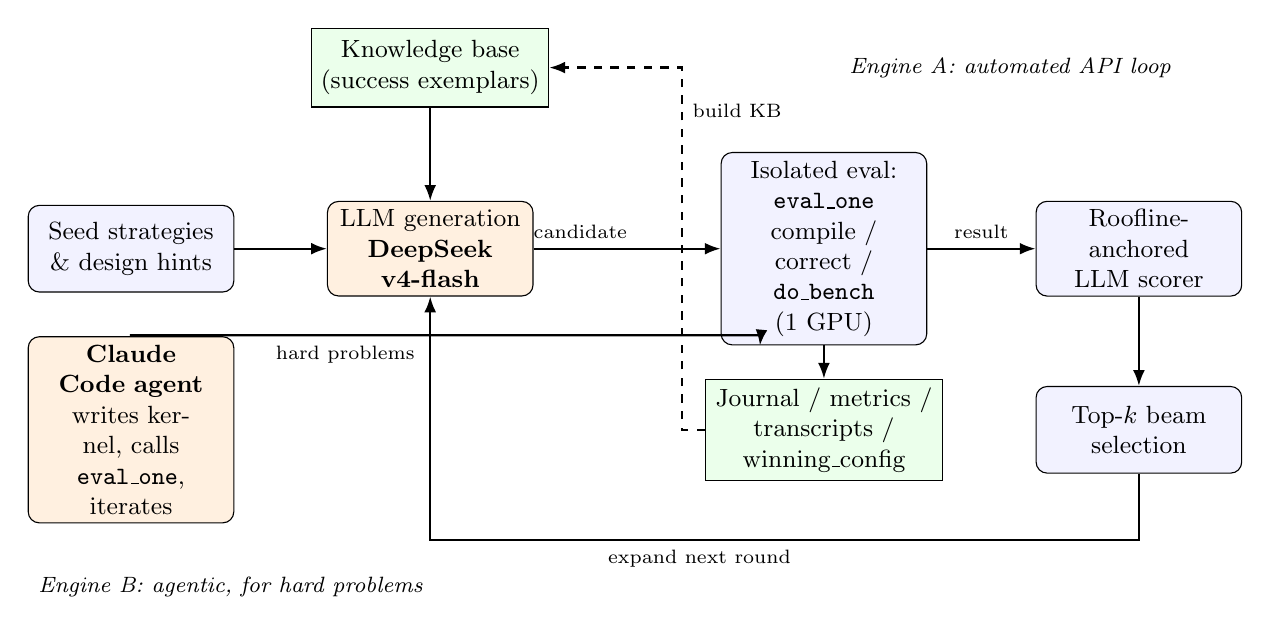
\begin{tikzpicture}[
    font=\small,
    box/.style={draw, rounded corners, align=center, text width=24mm,
                minimum height=11mm, inner sep=3pt, fill=blue!5},
    eng/.style={draw, rounded corners, align=center, text width=24mm,
                minimum height=11mm, inner sep=3pt, fill=orange!12},
    store/.style={draw, align=center, text width=28mm, minimum height=10mm,
                  inner sep=3pt, fill=green!8},
    arr/.style={-{Latex[length=2mm]}, thick},
  ]

  % main row (y=0); eval/score pushed right to lengthen the gen->eval arrow
  \node[box] (seed)  at (0,0)     {Seed strategies \\ \& design hints};
  \node[eng] (gen)   at (3.8,0)   {LLM generation \\ \textbf{DeepSeek v4-flash}};
  \node[box] (eval)  at (8.8,0)   {Isolated eval: \texttt{eval\_one} \\ compile / correct / \\ \texttt{do\_bench} (1 GPU)};
  \node[box] (score) at (12.8,0)  {Roofline-anchored \\ LLM scorer};

  % satellites
  \node[store] (kb)   at (3.8,2.3)  {Knowledge base \\ (success exemplars)};
  \node[store] (jrn)  at (8.8,-2.3) {Journal / metrics / \\ transcripts / winning\_config};
  \node[box]   (beam) at (12.8,-2.3){Top-$k$ beam \\ selection};
  \node[eng]   (agent) at (0,-2.3)  {\textbf{Claude Code agent} \\ writes kernel, calls \\ \texttt{eval\_one}, iterates};

  % straight links; "candidate" sits on the LEFT of the (now longer) arrow
  \draw[arr] (seed) -- (gen);
  \draw[arr] (gen)  -- node[above,font=\scriptsize,pos=0.25]{candidate} (eval);
  \draw[arr] (eval) -- node[above,font=\scriptsize]{result} (score);
  \draw[arr] (kb)   -- (gen);
  % eval -> journal leaves from the CENTER-bottom of eval
  \draw[arr] (eval.south) -- (jrn.north);
  \draw[arr] (score) -- (beam);

  % beam -> gen feedback ("expand"): down, left along the lowest band, up into gen
  \draw[arr] (beam.south) -- (12.8,-3.7) -- node[below,font=\scriptsize,pos=0.62]{expand next round}
        (3.8,-3.7) -- (gen.south);

  % journal -> KB feedback (dashed): up the RIGHT part of the gen--eval gap (x=7.0)
  \draw[arr,dashed] (jrn.west) -- (7.0,-2.3) -- node[right,font=\scriptsize,pos=0.88]{build KB}
        (7.0,2.3) -- (kb.east);

  % Claude agent -> eval ("hard problems"): across an empty band (y=-1.1) into the
  % SOUTH-WEST corner of eval, so it does not share the eval->journal start point.
  \draw[arr] (agent.north) -- (0,-1.1) -- node[below,font=\scriptsize,pos=0.34]{hard problems}
        (8.0,-1.1) -- ([xshift=5mm]eval.south west);

  % engine labels, clear of every box and routed line
  \node[font=\footnotesize\itshape, anchor=west] at (9.0,2.3)  {Engine A: automated API loop};
  \node[font=\footnotesize\itshape, anchor=west] at (-1.3,-4.3) {Engine B: agentic, for hard problems};

\end{tikzpicture}
}
  \caption{The closed-loop harness. Engine~A (DeepSeek API loop) and Engine~B
  (Claude Code agent) are two entry points into one shared evaluator; all
  persisted artifacts (logs, transcripts, winning configurations) are produced by
  the evaluator, not the generator.}
  \label{fig:pipeline}
\end{figure*}

\subsection{Prompt-engineering design}
The \emph{system prompt} fixes the role, the target hardware, the hard
constraints (define only \texttt{triton\_run}; no direct call to the reference
op; allowed imports; Triton~3.6 API pitfalls), and the required output format
(one Python block plus a confidence line). It is identical across candidates so
that DeepSeek's prefix cache is hit. The \emph{input prompt} is built per
candidate: operator signature, tolerance, the PyTorch reference source, the
assigned optimization strategy, the parent kernel and its measurement when
refining, and KB exemplars. Both are reproduced verbatim in
Appendices~\ref{app:input} and \ref{app:system}.

\subsection{Iteration strategy and two-layer search}
The outer loop explores \emph{algorithmic structure} (fusion, single-pass
reductions, persistent kernels, split-K). Within a candidate, tunable launch and
tile parameters are exposed as an LLM-chosen grid and swept by Triton's
autotuner; the evaluator records the winning configuration so the next round can
narrow the grid. A pilot showed that most of the gain comes from a good seed plus
a short error-fix loop, so we foreground a minimal tree with free repair and keep
the strategy/bandit/scorer mechanisms as ablation toggles.

\subsection{The agent-handoff contract (\texttt{HARNESS.md})}
The operators the API loop cannot solve are not left unsolved: we designed a
written contract that hands them to an agent (Fig.~\ref{fig:harness}). The
contract fixes three things. \emph{What the agent reads}: a task card with the
operator signature, tolerance, the PyTorch reference, forbidden patterns, and the
roofline target, plus KB exemplars and, for a resumed task, the handoff state
(\texttt{STATE.md}, \texttt{best.py}, and the journal tail). \emph{What the agent
writes}: one candidate file per attempt, an appended journal row through the same
\texttt{eval\_one} evaluator the API loop uses (so the results are directly
comparable), a \texttt{STATE.md} carrying status, what was tried, pitfalls, and
next steps for the following session, and a \texttt{best.py} exported from the
journal. \emph{Its iteration scope}: the budget is simply the journal line count,
and the agent loops write\,$\to$\,evaluate\,$\to$\,read (a traceback or a
measurement)\,$\to$\,refine until the budget is spent or the kernel saturates the
roofline. Because the agent calls the identical evaluator, its kernels are timed
and checked exactly like the API loop's, and both feed one comparison.

\begin{figure*}[t]
  \centering
  \resizebox{0.96\textwidth}{!}{% TikZ figure of the HARNESS.md agent-handoff contract: what the agent READS,
% what it WRITES, and its ITERATION scope. \input inside a figure* environment.
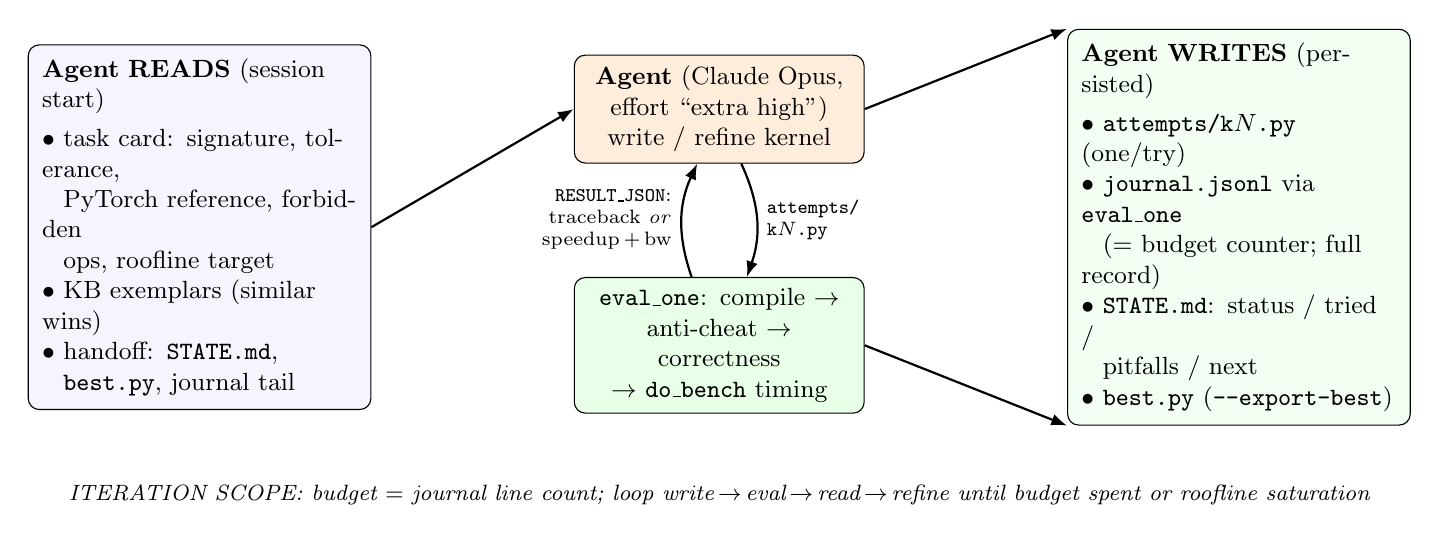
\begin{tikzpicture}[
    font=\small,
    panel/.style={draw, rounded corners, align=left, text width=40mm,
                  fill=blue!4, inner sep=5pt},
    agent/.style={draw, rounded corners, align=center, text width=34mm,
                  fill=orange!14, inner sep=4pt, minimum height=12mm},
    ev/.style={draw, rounded corners, align=center, text width=34mm,
               fill=green!9, inner sep=4pt, minimum height=12mm},
    arr/.style={-{Latex[length=2mm]}, thick},
  ]

  \node[panel] (reads) at (0,0) {\textbf{Agent READS} (session start)\\[3pt]
    $\bullet$ task card: signature, tolerance,\\ \phantom{$\bullet$} PyTorch reference, forbidden\\ \phantom{$\bullet$} ops, roofline target\\
    $\bullet$ KB exemplars (similar wins)\\
    $\bullet$ handoff: \texttt{STATE.md},\\ \phantom{$\bullet$} \texttt{best.py}, journal tail};

  \node[agent] (agent) at (6.6,1.5)
    {\textbf{Agent} (Claude Opus,\\ effort ``extra high'')\\ write / refine kernel};
  \node[ev] (eval) at (6.6,-1.5)
    {\texttt{eval\_one}: compile $\to$\\ anti-cheat $\to$ correctness\\ $\to$ \texttt{do\_bench} timing};
  \draw[arr] (agent) to[bend left=22]
        node[midway,right,font=\scriptsize,align=left]{\texttt{attempts/}\\\texttt{k$N$.py}} (eval);
  \draw[arr] (eval) to[bend left=22]
        node[midway,left,font=\scriptsize,align=right]{\texttt{RESULT\_JSON}:\\traceback \emph{or}\\ speedup\,+\,bw} (agent);

  \node[panel, fill=green!5] (writes) at (13.2,0)
    {\textbf{Agent WRITES} (persisted)\\[3pt]
    $\bullet$ \texttt{attempts/k$N$.py} (one/try)\\
    $\bullet$ \texttt{journal.jsonl} via \texttt{eval\_one}\\ \phantom{$\bullet$} ($=$ budget counter; full record)\\
    $\bullet$ \texttt{STATE.md}: status / tried /\\ \phantom{$\bullet$} pitfalls / next\\
    $\bullet$ \texttt{best.py} (\texttt{-{}-export-best})};

  \draw[arr] (reads.east) -- (agent.west);
  \draw[arr] (agent.east) -- (writes.north west);
  \draw[arr] (eval.east) -- (writes.south west);

  \node[align=center, font=\footnotesize\itshape] at (6.6,-3.4)
    {ITERATION SCOPE: budget $=$ journal line count; loop write\,$\to$\,eval\,$\to$\,read\,$\to$\,refine
     until budget spent or roofline saturation};
\end{tikzpicture}
}
  \caption{The \texttt{HARNESS.md} agent-handoff contract: what the agent reads at
  the start of a session, what it writes (all through the same \texttt{eval\_one}
  evaluator as Engine~A), and its iteration scope. This is how operators that the
  one-shot API loop cannot solve are completed by an agent.}
  \label{fig:harness}
\end{figure*}

%------------------------------------------------------------------------------
\section{Experimental Setup}
All measurements come from one evaluator run as an isolated subprocess bound to a
single GPU via \texttt{CUDA\_VISIBLE\_DEVICES}, so exactly one candidate is timed
per card at a time. Both the candidate and the PyTorch reference are timed with
\texttt{triton.testing.do\_bench} (median over 100 reps after 25 warmups), and
both include output allocation, removing an asymmetry that would flatter the
kernel. Correctness uses \texttt{torch.allclose} at per-operator tolerances
against the eager reference with a fixed input seed. Hardware is an NVIDIA
RTX~5090 (Blackwell, sm\_120, 32\,GB GDDR7, $\sim$1790~GB/s peak); software is
PyTorch (CUDA 12.8) with Triton 3.6. A static anti-cheat check rejects candidates
that call the reference op directly (tagged \texttt{cheat}). We define
\textbf{success} as a candidate that is correct within tolerance and faster than
eager ($\text{speedup}>1$); a \textbf{failure} is any incorrect, non-compiling,
timed-out, or cheating candidate. Every run writes a per-candidate
\texttt{journal.jsonl} (the single source of truth: correctness, speedup,
bandwidth, winning configuration, token/GPU cost, full code) plus round metrics
and full LLM transcripts; all tables and figures here are generated from those
logs with no hand-entered numbers.

%------------------------------------------------------------------------------
\section{Results}
On the memory-bound suite the API loop delivers large, defensible speedups
(Fig.~\ref{fig:dsbar}). The operators whose references waste the most memory
traffic win biggest: KL-divergence at $4.61\times$ and RoPE at $4.29\times$,
followed by Welford ($2.43\times$), RMSNorm ($2.32\times$), and cross-entropy
($2.18\times$), each by fusing a multi-pass reference into one pass. The five
control operators land at $0.99$--$1.07\times$: the engine correctly finds no
headroom where the reference already saturates bandwidth. Across 222 candidates
on 14 operators, 74\% were correct and 43\% of operators cleared $1.2\times$
(Table~\ref{tab:ds}). Best results for all 17 operators in the suite---including
\texttt{swiglu} and \texttt{addmm}, not otherwise plotted---are in
Appendix~\ref{app:allops}.

\begin{figure}[t]
  \centering
  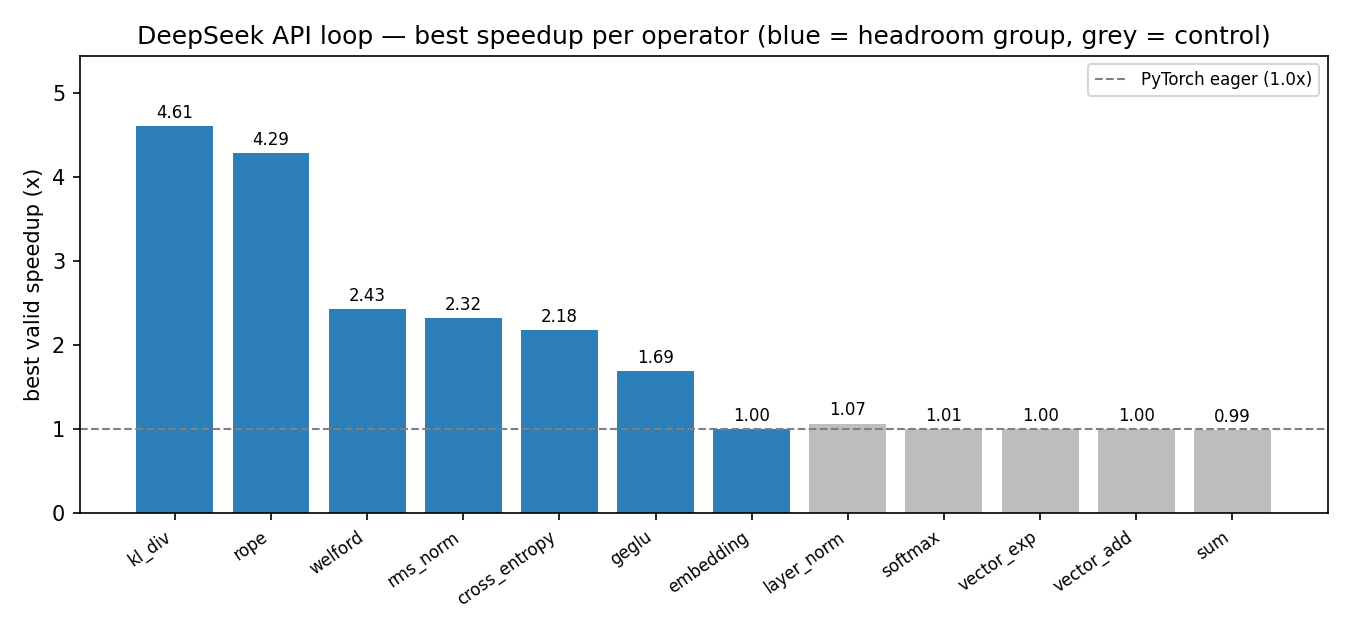
\includegraphics[width=\columnwidth]{figures/deepseek_speedup.png}
  \caption{DeepSeek API loop: best valid speedup per operator over PyTorch eager.
  Blue: headroom group; grey: control group at the memory roofline.}
  \label{fig:dsbar}
\end{figure}

\begin{table}[t]
  \centering \footnotesize
  \caption{DeepSeek API-loop totals (14 operators).}
  \label{tab:ds}
  \begin{tabular}{lrl}
    \toprule
    Metric & Value & Unit \\
    \midrule
    Candidates generated            & 222  & kernels \\
    Passed correctness              & 74   & \% of candidates \\
    Operators with $>\!1\times$ speedup    & 71 & \% of operators \\
    Operators with $>\!1.2\times$ speedup  & 43 & \% of operators \\
    GPU evaluation time             & 15.4 & minutes \\
    LLM tokens used                 & 1.52 & million \\
    \bottomrule
  \end{tabular}
\end{table}

The agentic engine was pointed at \texttt{int4\_gemm}: a 4-bit weight, fp16
activation matrix multiply that must dequantize packed weights inside the kernel,
beating a baseline that dequantizes to a full fp16 matrix and calls cuBLAS. Its
first two attempts failed; the third was correct at $0.99\times$, and it then
climbed a tuning ladder to $1.09\times$ (Fig.~\ref{fig:ladder}). The decisive
moves were structural---dropping a 3-D reshape and loading weights as a
\texttt{[BLOCK\_K,BLOCK\_N]} tile via redundant, L2-cached rows---and a launch
sweep settling on a $128\!\times\!64\!\times\!64$ tile, \texttt{GROUP\_M}=4,
\texttt{num\_warps}=8, \texttt{num\_stages}=2. At $1.09\times$ the kernel sits at
$\approx 89\%$ of fp16 tensor-core peak; the agent declared saturation by a
hardware-limit argument rather than spending more budget.

\begin{figure}[t]
  \centering
  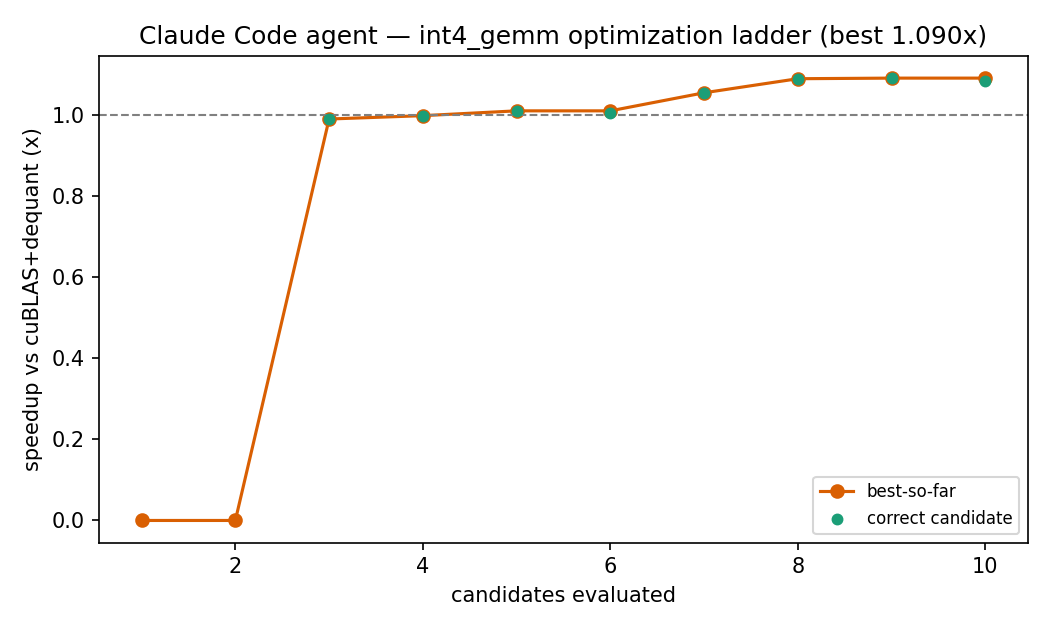
\includegraphics[width=0.82\columnwidth]{figures/int4gemm_ladder.png}
  \caption{Claude Code agent on \texttt{int4\_gemm}: best-so-far speedup over a
  cuBLAS+dequantize baseline. Two failed attempts, then a correct kernel and a
  tuning ladder to $1.09\times$.}
  \label{fig:ladder}
\end{figure}

The engines diverge sharply on the hardest, compute-bound operators
(Table~\ref{tab:h2h}). On \texttt{int4\_gemm} the API loop produced 12 candidates
and none were correct; the agent reached $1.09\times$. The pattern repeats on the
other hard operators. On fused-linear cross-entropy (\texttt{flce}) the flash API
loop produced 0 of 12 correct and pro managed only $1.21\times$, whereas the agent
reached about $5\times$ (best $5.1\times$, independently re-measured at $4.6\times$
on an idle GPU) by fusing the logit reduction so the 268\,MB logit tensor is never
materialized. On plain \texttt{gemm} no engine beats cuBLAS: the agent's best
($1.01\times$, 9/14 correct) merely matches it, as expected for an already-optimal
fp16 GEMM. The hard kernels reward the agent's compile--read--repair loop.

\subsection{Scaling the generator: flash vs.\ pro}
To test whether the API loop's failures are simply a matter of a weak model, we
re-ran it with the larger \textsc{DeepSeek-v4-pro} at two budgets, 12 and 24
candidates per operator. On memory-bound operators flash and pro are tied, and the
extra budget barely moves the result (Table~\ref{tab:pro}): KL-divergence stays at
$4.61\times$, cross-entropy at $2.18\times$, and the rest within a few percent. The
only visible budget effect is \texttt{welford}, where pro rises from $2.17$ to
$2.42\times$ as more attempts lift its correctness rate. The ceiling here is the
shared roofline, not the model or the budget. (Pro$\,$(24) was re-timed on an
exclusive GPU; an earlier shared-GPU run had contention-inflated references and is
discarded---timing requires an exclusive card.) The larger model does help on one
hard case---it cracked \texttt{flce} (2/8 correct, $1.21\times$)
where flash got 0/12---but \texttt{int4\_gemm} remained 0/12 for \emph{both}
models, and \texttt{gemm}/\texttt{addmm} stayed below the cuBLAS baseline. Scaling
the single-shot generator does not close the gap that the agent closes (the agent
reaches $5\times$ on \texttt{flce} and $1.09\times$ on \texttt{int4\_gemm}).

\begin{table}[t]
  \centering \footnotesize
  \caption{Head-to-head on the hardest operators (correct/attempts; best speedup
  where any candidate is correct).}
  \label{tab:h2h}
  \begin{tabular}{lcccc}
    \toprule
    Operator & DS-flash & DS-pro & Claude (B) & Best \\
    \midrule
    \texttt{int4\_gemm} & 0/12 & 0/12 & 8/10\,@1.09 & \textbf{1.09$\times$} (B) \\
    \texttt{flce}       & 0/12 & 2/8\,@1.21 & 6/7\,@5.1 & \textbf{5.1$\times$} (B) \\
    \texttt{gemm}       & 0/12 & 3/12\,@0.94 & 9/14\,@1.01 & 1.01$\times$ (B) \\
    \bottomrule
  \end{tabular}
\end{table}

\begin{table}[t]
  \centering \footnotesize
  \caption{Memory-bound operators: best speedup for \textsc{DeepSeek}-flash and
  -pro at candidate budgets of 12 and 24. Numbers in parentheses are the column
  header budgets; pro$\,$(24) was re-timed on an exclusive GPU. Flash and pro are
  tied, and raising the pro budget from 12 to 24 changes little.}
  \label{tab:pro}
  \begin{tabular}{lccc}
    \toprule
    Operator & flash$\,$(24) & pro$\,$(12) & pro$\,$(24) \\
    \midrule
    \texttt{rope}          & 4.29$\times$ & 4.41$\times$ & 3.96$\times$ \\
    \texttt{kl\_div}       & 4.61$\times$ & 4.60$\times$ & 4.61$\times$ \\
    \texttt{rms\_norm}     & 2.32$\times$ & 2.30$\times$ & 2.30$\times$ \\
    \texttt{cross\_entropy}& 2.18$\times$ & 2.11$\times$ & 2.18$\times$ \\
    \texttt{welford}       & 2.43$\times$ & 2.17$\times$ & 2.42$\times$ \\
    \texttt{geglu}         & 1.69$\times$ & 1.68$\times$ & 1.68$\times$ \\
    \bottomrule
  \end{tabular}
\end{table}

%------------------------------------------------------------------------------
\section{Discussion and Analysis}
The central finding is complementarity, and the failures explain why. We did a
root-cause analysis of the cases where Engine~A failed.

\textbf{Why \texttt{int4\_gemm} failed for the API loop (0/12).} The errors split
across three causes recorded in the logs. \emph{Runtime} errors dominated: the
kernel must unpack eight 4-bit weights from each 32-bit word with bit shifts and
masks, align them to the K-loop, and subtract the zero point---an indexing
problem the single-shot model got wrong (out-of-bounds and dtype mismatches). One
candidate produced \emph{wrong output} (a correct-looking but mis-scaled
dequantization), and several were rejected as \emph{cheat} for falling back to a
high-level matmul. The task needs several interdependent steps to be correct
simultaneously; a generator with no feedback rarely lands all of them at once.
The agent succeeded precisely because it could compile, read the traceback, and
fix one cause at a time.

\textbf{Why fused-linear cross-entropy failed for the API loop, and how the agent
won.} For flash all 12 failures were runtime errors; pro got it correct twice but
only to $1.21\times$. The operator fuses a matmul with a logsumexp and a gathered
negative log-likelihood without materializing the full logits; getting the tiled
online reduction and the target gather correct in one shot is beyond the
single-pass generator. The agent, iterating, reached about $5\times$---the largest
single win in the suite---because the fused kernel never writes the 268\,MB logit
tensor that the eager reference materializes. This is the clearest case for the
agentic engine: the same problem that yields 0/12 to one-shot generation is a
$5\times$ win once the loop can repair and refine.

\textbf{Is it just a weak model?} No. Replacing flash with the larger pro model
left memory-bound speedups unchanged (the roofline, not the model, is the limit
there) and still produced 0/12 correct on \texttt{int4\_gemm}. The bigger model
did crack \texttt{flce} ($1.21\times$), so model capacity helps at the margin on
hard problems---but the decisive factor for the hardest kernel was the agent's
ability to compile, read the error, and fix one cause at a time, not raw model
strength.

\textbf{Where the API loop wins.} Memory-bound operators reward a single good
idea---fuse the passes---that the model already knows from the Liger family;
correctness is then easy and the speedup follows. Budget curves (not shown) place
most of the gain in the first few candidates, which argues for spending budget on
seed diversity and fast repair rather than deep refinement. The control group
matters: reporting $\approx 1.0\times$ where the roofline leaves no room is what
makes the large speedups credible.

\textbf{Threats to validity.} Speedups are measured on one GPU and one input
shape per operator; the roofline uses a vendor peak rather than a measured stream
ceiling; and the agent result covers a single operator.

%------------------------------------------------------------------------------
\section{Conclusion}
An LLM-in-the-loop tree search over Triton kernels yields real, verified speedups
on memory-bound operators ($2$--$4.6\times$) at a total cost near \$1. The choice
of driver matters: a cheap API loop is the right tool for fuse-the-passes
problems, while a hard compute-bound kernel like 4-bit GEMM needs an agent that
can reason across steps and repair its own errors. The two engines are
complementary, and the failure analysis---not just the speedups---is the useful
product.

\section*{Acknowledgment}
Kernels were generated by \textsc{DeepSeek-v4-flash} and \textsc{Claude Code} as
the object of study; reported numbers trace to the run logs in the project
repository.

\bibliographystyle{IEEEtran}
\bibliography{refs}

% ---- end of main body + references; Appendix below is NOT counted (6-pp limit).
\xdef\mainbodyendpage{\thepage}

%==============================================================================
%  APPENDIX -- REQUIRED RAW MATERIALS (Category B)
%==============================================================================
\appendices

\section{Complete Per-Operator Results}
\label{app:allops}
All 17 operators in the suite were run through the harness.
Table~\ref{tab:allops} gives the best valid speedup for each and the engine that
achieved it. 16 of 17 reached a correct kernel; only \texttt{addmm} (fp16
bias-plus-matmul against cuBLAS) produced no correct candidate, like the other
matmul kernels that cannot beat cuBLAS. Memory-bound figures are the
\textsc{DeepSeek}-flash values from the main results (clean, exclusive-GPU
timing); \texttt{swiglu} was only run with \textsc{DeepSeek}-pro.

\begin{table}[h]
  \centering \footnotesize
  \caption{Best valid speedup over PyTorch eager for every operator in the
  17-operator suite, and the engine that achieved it (DeepSeek API loop vs.\
  Claude agent).}
  \label{tab:allops}
  \begin{tabular}{llrl}
    \toprule
    Operator & Category & Best & Engine \\
    \midrule
    \multicolumn{4}{@{}l}{\emph{Memory-bound, with headroom}}\\
    \texttt{rope}          & positional    & 4.29$\times$ & DeepSeek \\
    \texttt{kl\_div}       & loss          & 4.61$\times$ & DeepSeek \\
    \texttt{welford}       & reduction     & 2.43$\times$ & DeepSeek \\
    \texttt{rms\_norm}     & normalization & 2.32$\times$ & DeepSeek \\
    \texttt{cross\_entropy}& loss          & 2.18$\times$ & DeepSeek \\
    \texttt{geglu}         & elementwise   & 1.69$\times$ & DeepSeek \\
    \texttt{swiglu}        & elementwise   & 1.67$\times$ & DeepSeek \\
    \texttt{embedding}     & positional    & 1.00$\times$ & DeepSeek \\
    \midrule
    \multicolumn{4}{@{}l}{\emph{Memory-bound, at the roofline (control)}}\\
    \texttt{layer\_norm}   & normalization & 1.07$\times$ & DeepSeek \\
    \texttt{softmax}       & normalization & 1.01$\times$ & DeepSeek \\
    \texttt{vector\_add}   & elementwise   & 1.00$\times$ & DeepSeek \\
    \texttt{vector\_exp}   & elementwise   & 1.00$\times$ & DeepSeek \\
    \texttt{sum}           & reduction     & 0.99$\times$ & DeepSeek \\
    \midrule
    \multicolumn{4}{@{}l}{\emph{Compute-bound (hard)}}\\
    \texttt{flce}          & loss          & 5.15$\times$ & Claude agent \\
    \texttt{int4\_gemm}    & matmul        & 1.09$\times$ & Claude agent \\
    \texttt{gemm}          & matmul        & 1.01$\times$ & Claude agent \\
    \texttt{addmm}         & matmul        & ---          & none \\
    \bottomrule
  \end{tabular}
\end{table}

\section{Input Prompt}
\label{app:input}
Verbatim per-candidate input prompt for the RoPE operator (the run that produced
the $4.29\times$ result in Fig.~\ref{fig:dsbar}). For Engine~B (Claude Code, model
\textsc{Claude Opus}, reasoning effort ``extra high'') the user prompt is the
one-line task ``Read HARNESS.md, optimize int4\_gemm, budget 28 evals, use
GPU~N,'' with \texttt{HARNESS.md} as the standing system contract.
\lstinputlisting{appendix/input_prompt.txt}

\section{System Prompt}
\label{app:system}
Verbatim system prompt (identical across all Engine~A candidates; the cached
prefix).
\lstinputlisting{appendix/system_prompt.txt}

\section{Representative Agent Output}
\label{app:output}
Verbatim model response for the RoPE candidate above (the generated kernel,
$4.29\times$). The model also emits a one-line confidence record consumed by the
harness.
\lstinputlisting{appendix/agent_output.txt}

\noindent The best Engine~B kernel (\texttt{int4\_gemm}, $1.09\times$) is included
in the repository at \texttt{runs/agent\_int4\_gemm/best.py}.

\section{Changes Made to the Agent}
We modified the harness and the agent contract during the project. (1)
\emph{Parameter-grid autotuning}: candidates now expose each tunable launch
parameter as an LLM-chosen grid swept by \texttt{triton.autotune}, and the
evaluator scans the autotuner to record the winning configuration in the log so
later rounds narrow the grid. (2) \emph{Transcript logging}: every LLM exchange
(system prompt, input prompt, raw response, and the model's reasoning) is saved
per candidate---these files are the source of this appendix. (3) \emph{Model
override}: a \texttt{--model} flag selects \textsc{DeepSeek-v4-pro} vs
\texttt{-flash} per run, recorded in the run metadata. (4) \emph{Multi-process
safety}: a spawn stagger and an optional startup jitter prevent simultaneous
CUDA-context initialization from many evaluator subprocesses. (5) \emph{Agent
contract} (\texttt{HARNESS.md}, Engine~B): the agent (\textsc{Claude Code}, model
\textsc{Claude Opus}, reasoning effort ``extra high'') writes a kernel, calls the
evaluator (\texttt{eval\_one}) with a strategy label, and hands off state through
a log-derived best kernel rather than conversation memory. The complete
\texttt{HARNESS.md} and configuration files are in the repository.

\end{document}
